\documentclass[12pt,a4paper]{article}
% !TEX program = xelatex
\usepackage[utf8]{inputenc}
\usepackage[T1]{fontenc}
\usepackage[finnish]{babel}
\usepackage[utf8]{inputenc}
\usepackage{graphicx}
\usepackage{titling}
\usepackage{titlesec}
\usepackage{booktabs}
\usepackage{fancyhdr}
\usepackage{lipsum}
\usepackage{comment}
\usepackage{enumitem}
\usepackage{xcolor}
\usepackage{longtable}
%\usepackage{cite}
\usepackage{pgfgantt}
\usepackage{amsmath, amssymb}
\usepackage{tikz}
\usepackage[margin=1in]{geometry}
\usepackage[backend=biber, style=numeric]{biblatex}
%\usepackage{hyperref}
\usepackage{bookmark}
\usepackage{enumitem}
\usepackage{amsmath}
\usepackage{listings}
\lstset{language=Python, basicstyle=\ttfamily\small, breaklines=true,columns=fullflexible}
\lstset{escapeinside={(*@}{@*)}}
\usepackage{fontspec}
\setmainfont{Arial}
\newfontfamily\stylishfont{Noteworthy}
%\newfontfamily\stylishfont{Zapfino}
%\addbibresource{references.bib}
\usetikzlibrary{calc}
\usepackage{xcolor}

\lstdefinestyle{pidstyle}{
    basicstyle=\ttfamily\footnotesize,
    breaklines=true,
    escapechar=\#, % Define escape character for inline LaTeX commands
    linewidth=\textwidth,
    basicstyle=\ttfamily\scriptsize
}

\renewcommand{\maketitle}{%
  \begin{leftmark}
    \vspace*{\baselineskip} % Add a bit of vertical space

%    \includegraphics[width=4cm]{example-image-a} % Add an image before the title. you will need to replace the image path with your own

%    \vspace{0.5cm} % Add vertical space before title

    \textbf{\fontsize{18}{36}\selectfont \thetitle} % Font Size and Bold Title

     \vspace{0.05cm} % Add vertical space before subtitle
%    \textit{\Large \theauthor}  % Subtitle / Author
    \vspace{\baselineskip} % Add vertical space after subtitle
     \rule{\textwidth}{0.4pt} % Add a horizontal line

   \end{leftmark}
%    \thispagestyle{empty} % Prevent header/footer on the title page
}


% Section Formatting
\titleformat{\section}
  {\normalfont\fontsize{18}{22}\bfseries} % Font and style
  {\thesection}         % Section number
  {1em}                   % Horizontal space after section number
  {}                     % Code before the section name
  []                     % Code after the section name

\titleformat{\subsection}
  {\normalfont\fontsize{14}{18}\bfseries} % Font and style
  {\thesubsection}         % Subsection number
  {1em}                   % Horizontal space after subsection number
  {}                     % Code before the subsection name
  []                     % Code after the subsection name

\setlength{\parindent}{0pt}

\title{Computing platforms (Spring 2025)\newline
week 6}
\author{Juha-Pekka Heikkilä}



\pagestyle{fancy}
\fancyhf{}

\renewcommand{\headrulewidth}{0pt}

\newcommand{\footerline}{\makebox[\textwidth]{\hrulefill}}

\newcommand{\footercontent}{%
    \begin{tabular}{@{}l@{}}
        \footerline \\
        \leftmark \hfill \rlap{\thepage}
    \end{tabular}
}

\fancyfoot[C]{\footercontent}


\newcommand{\exercise}[1]{
    \section*{Tehtävä #1}
    \markboth{Tehtävä #1}{}
}

\addtolength{\hoffset}{-1.75cm}
\addtolength{\textwidth}{3.5cm}
%\addtolength{\voffset}{-3cm}
%\addtolength{\textheight}{6cm}
%\setlength{\parindent}{0pt}



% (a), (b), (c)
\newlist{kohta}{enumerate}{1}
\setlist[kohta,1]{
  label=\textbf{\makebox[1cm][l]{\Huge\text{(\stylishfont\alph*)}}},
  leftmargin=!,
  labelindent=0pt
}

% (1), (2), (3)
\newlist{alakohta}{enumerate}{1}
\setlist[alakohta,1]{
  label=\textbf{\makebox[1cm][l]{\Large\text{(\arabic*)}}},
  leftmargin=!,
  labelindent=0pt
}

% termi: selitys
\newlist{kuvaus}{description}{1}
\setlist[kuvaus]{%
  font=\bfseries\stylishfont,
  labelsep=0.5cm,
  leftmargin=2.5cm,
  style=nextline
}

\newcommand{\korostus}[2][yellow]{\colorbox{#1}{\strut #2}}
%\korostus{Yksi kirjoittaja on jo sisällä}
%\korostus[red]{Lukijan täytyy odottaa jos kirjoittajia on paikalla}
%\korostus[orange]{Tämä osa ei ole suoritettavissa}


\newcommand{\evalslantti}[4][-12]{%
%  \left. #2 \,\right|% ei indeksejä tähän
  \mkern-10mu\raisebox{0pt}[0pt][0pt]{\rotatebox{#1}{$\Big|$}}% vinoviiva päälle
  \mkern3mu{}_{\!#3}^{\!#4}% arvot viivan oikealle puolelle
}



\newcommand{\evalraise}{1.2ex}
\newcommand{\evallow}{1.2ex}

% vino eval-viiva, arvot oikealla (oletus: -12)
% \evalslant[asteet]{lauseke}{ala}{yla}
\newcommand{\evalslant}[4][-12]{%
  \left. #2 \,\right.%
  \mkern-10mu\raisebox{0pt}[0pt][0pt]{\rotatebox{#1}{$\Big|$}}%
  \mkern2mu{}^{\raisebox{\evalraise}{$\scriptstyle #4$}}_{\raisebox{-\evallow}{$\scriptstyle #3$}}%
}
\newcommand{\riip}{\perp \!\!\! \perp}

\title{MAT12003 Todennäköisyyslaskenta I — Viikko 3}
\date{}

\begin{document}

\maketitle

\exercise{1}
Heitetään kahta noppaa. Olkoon $A =$ ”ainakin toinen silmäluvuista on parillinen” ja $B =$ ”silmälukujen summa on vähintään 9”. Ovatko $A$ ja $B$ riippumattomia?


\vspace{0.4cm}


Perusjoukko $|\Omega|=36$.

\[
P(A)=1-\Big(\tfrac36\Big)^2=\tfrac{27}{36}=\tfrac34,\qquad
P(B)=\tfrac{10}{36}=\tfrac{5}{18}
\]
summaa $\ge 9$ on 10 tapausta ja niistä vain $(5,5)$ ei kuulu $A$:han

{\small
\[
\begin{array}{c|l|c|c}
\text{Summa} & \text{tulokset} & \# & \text{väh. yksi parillinen}\\
\hline
9  & (3,6),(4,5),(5,4),(6,3) & 4 & 4 \\
10 & (4,6),(5,5),(6,4)       & 3 & 2 \\
11 & (5,6),(6,5)             & 2 & 2 \\
12 & (6,6)                   & 1 & 1 \\
\hline
   & \text{yhteensä}         & 10& 9
\end{array}
\]}

joten
\[
P(A\cap B)=\tfrac{9}{36}=\tfrac14
\]
Koska
\[
P(A)P(B)=\tfrac34\cdot\tfrac{5}{18}=\tfrac{5}{24}\ \ne\ \tfrac14=P(A\cap B)
\]
\vspace{0.4cm}

tapahtumat $A$ ja $B$ eivät ole riippumattomia.







\pagebreak
\exercise{2}
Korttipakasta nostetaan 13 korttia (ilman takaisinpanoa). Olkoon $X$ ässien lukumäärä otoksessa. Laske tapahtumien $\{X=3\}$ ja $\{X\ge 2\}$ todennäköisyydet. Mitä jakaumaa $X$ noudattaa?
\vspace{0.4cm}

Koska nostot tehdään ilman takaisinpanoa populaatiosta
(N=52) jossa on K=4 ässää, ässien lukumäärä X noudattaa
hypergeometrista jakaumaa: $X\sim\mathrm{Hyperg}(52,4,13)$
\vspace{0.4cm}

\[
P(X=k)=\frac{\binom{4}{k}\,\binom{48}{13-k}}
{\binom{52}{13}},\qquad k=0,1,2,3,4
\]

\begin{kohta}
\item $P(X=3)$:
\[
P(X=3)=\frac{\binom{4}{3}\binom{48}{10}}{\binom{52}{13}}
=\frac{858}{20825}\approx 0{,}04120
\]

\item $P(X\ge 2)$ (komplementtina):
%\[
%f(k\ge 2) = P(X\ge 2)=1-P(X\le 1)
%=1-\frac{\binom{48}{13}+\binom{4}{1}\binom{48}{12}}{\binom{52}{13}}
%=\frac{5359}{20825}\approx 0{,}25733
%\]

\[ P(X \ge 2) = 1 - P(X \le 1) = 1 - \big( P(X=0) + P(X=1) \big) \]
\[ 
\begin{aligned}
&= 1 - \left( \frac{\binom{4}{0}\binom{48}{13}}{\binom{52}{13}} + \frac{\binom{4}{1}\binom{48}{12}}{\binom{52}{13}} \right)\\
&=\frac{5359}{20825}\approx 0{,}25733
\end{aligned}
\]
\end{kohta}





\pagebreak
\exercise{3}
Olkoot $A$, $B$ ja $C$ tapahtumia, joille $P(A)=P(B)=0{,}25$ ja $P(C)=0{,}3$. Lisäksi tiedetään, että $A\riip B$ ja $B\riip C$ sekä $A$ ja $C$ ovat erillisiä. Laske $P(A\cup B\cup C)$.\\

\noindent Vinkki: Muista, että $A\cup B\cup C=(A\cup B)\cup C$ ja $(A\cup B)\cap C=(A\cap B)\cup(B\cap C)$.


\begin{alakohta}
\item Hajotus ja leikkauksen lasku:
\[
A\cup B\cup C=(A\cup B)\cup C,\qquad
(A\cup B)\cap C=(A\cap C)\cup(B\cap C)
\]
Koska $A$ ja $C$ ovat erillisiä, $A\cap C=\varnothing$, joten
\[
(A\cup B)\cap C = B\cap C
\]

\item $P(A\cup B)$ riippumattomuudesta:
\[
P(A\cup B)=P(A)+P(B)-P(A\cap B),
\quad A\riip B\Rightarrow P(A\cap B)=P(A)P(B)=\tfrac14\cdot\tfrac14=\tfrac{1}{16}
\]
Siis:
\[
P(A\cup B)=\tfrac14+\tfrac14-\tfrac{1}{16}=\tfrac{7}{16}
\]

\item $P(B\cap C)$ riippumattomuudesta:
\[
B\riip C\Rightarrow P(B\cap C)=P(B)P(C)=\tfrac14\cdot\tfrac{3}{10}=\tfrac{3}{40}
\]

\item Edelliset yhdessä:
\[
\begin{aligned}
P(A\cup B\cup C)
&=P(A\cup B)+P(C)-P\big((A\cup B)\cap C\big)\\
&=\tfrac{7}{16}+\tfrac{3}{10}-\tfrac{3}{40}
= \frac{35+24-6}{80}
= \frac{53}{80}
=0{,}6625
\end{aligned}
\]
\end{alakohta}







\pagebreak
\exercise{4}
Heitetään painotettua kolikkoa kolme kertaa. Heitot ovat riippumattomia toisistaan, ja kruunan todennäköisyys on $p$, ($0<p<1$). Osoita, että tapahtumat
\begin{align*}
A&=\text{''saadaan sekä kruunia että klaavoja''},\\
B&=\text{''saadaan enintään yksi klaava''}
\end{align*}
ovat riippumattomia, jos ja vain jos $p=\frac{1}{2}$.


\begin{alakohta}
\item Perustodennäköisyydet:
\[
P(A)=1-\big(p^3+(1-p)^3\big)=3p(1-p)
\]
(A: vähintään yksi kumpaakin \Leftrightarrow \, ei ole
kolme kruunaa eikä kolme klaavaa)

\[
P(B)=P(\text{0 klaavaa})+P(\text{1 klaava})
= p^3+3p^2(1-p)=p^2(3-2p)
\]

\[
P(A\cap B)=P(\text{täyttyy $A$ ja $\le1$ klaavaa})
= P(\text{tasan 1 klaava})
=3p^2(1-p)
\]

\item Riippumattomuusehto:\\ $A\riip B \iff P(A\cap B)=P(A)P(B)$
\[
3p^2(1-p)\;=\; \big(3p(1-p)\big)\,\big(p^2(3-2p)\big)
\quad\Longleftrightarrow\quad
1=p(3-2p)
\]
koska $0<p<1$ \Rightarrow \, voidaan jakaa tekijällä $3p^2(1-p)>0$\\
Tästä
\[
3p-2p^2=1\ \Longleftrightarrow\ 2p^2-3p+1=0
\ \Longleftrightarrow\ (2p-1)(p-1)=0
\]
Sallitulla välillä ratkaisu on \(p=\tfrac12\)

\item Takaisinpäin ("vain jos"): \\Kun \(p=\tfrac12\):
\[
P(A)=3\cdot\tfrac12\cdot\tfrac12=\tfrac34,\quad
P(B)=\tfrac14(3-1)=\tfrac12,\quad
P(A\cap B)=3\cdot\tfrac14\cdot\tfrac12=\tfrac38=\tfrac34\cdot\tfrac12
\]
Siis \(P(A\cap B)=P(A)P(B)\), joten \(A\riip B\)
\end{alakohta}

\noindent Siis: \(A\) ja \(B\) ovat riippumattomia jos ja 
vain jos \(p=\tfrac12\)










\pagebreak
\exercise{5}
Heitetään ensin tavallista 6-sivuista noppaa, sitten 
4-sivuista noppaa (jossa silmäluvut 1, 2, 3, 4 ovat yhtä todennäköiset).
Olkoon heittojen tulokset $X$ ja $Y$, ja $S=|X-Y|$. Laske satunnaismuuttujan $S$ pistetodennäköisyydet ja piirrä pistetodennäköisyysfunktiota havainnollistava pylväsdiagrammi sekä kertymäfunktion kuvaaja.\\




Kaikkia pareja on $6\cdot 4=24$. S saa arvot $s\in\{0,1,2,3,4,5\}$\\

\textbf{Pistetodennäköisyysfunktio (ptnf):}
Merkitään $p_S(s)=P(S=s)$
\[
p_S(s)=\frac{\#\{(x,y):|x-y|=s\}}{24}
\]

\emph{miksi nämä lukumäärät:} 
ehto $|x-y|=s$ tarkoittaa joko $x-y=s$ tai $y-x=s$:

{\small
\[
\begin{array}{c|c|c|c|c}
s & \#\{(x,y):x-y=s\} & \#\{(x,y):y-x=s\} & \text{yht.} & p_S(s)=\dfrac{\#}{24} \\\hline
0 & \#\{(1,1),(2,2),(3,3),(4,4)\}=4 & \text{--} & 4 & \dfrac{4}{24} \\
1 & 4 & 3 & 7 & \dfrac{7}{24} \\
2 & 4 & 2 & 6 & \dfrac{6}{24} \\
3 & 3 & 1 & 4 & \dfrac{4}{24} \\
4 & 2 & 0 & 2 & \dfrac{2}{24} \\
5 & 1 & 0 & 1 & \dfrac{1}{24} \\
\end{array}
\]
}
\begin{comment}
   
\begin{itemize}[leftmargin=1.2cm]
  \item $s=0$: parit $(1,1),(2,2),(3,3),(4,4)$ $\Rightarrow$ $\#=4$.
  \item $s=1$: $x-y=1$ tuottaa $x=2,3,4,5$ (4 kpl), ja $y-x=1$ tuottaa $y=2,3,4$ (3 kpl) $\Rightarrow$ $\#=7$.
  \item $s=2$: vastaavasti $4+2=6$.
  \item $s=3$: $3+1=4$.
  \item $s=4$: $2+0=2$.
  \item $s=5$: $1+0=1$.
\end{itemize}
\end{comment}

Siis ptnf on
\[
\begin{aligned}
p_S(0)&=\tfrac{4}{24}=\tfrac{1}{6},&
p_S(1)&=\tfrac{7}{24},&
p_S(2)&=\tfrac{6}{24}=\tfrac{1}{4},\\
p_S(3)&=\tfrac{4}{24}=\tfrac{1}{6},&
p_S(4)&=\tfrac{2}{24}=\tfrac{1}{12},&
p_S(5)&=\tfrac{1}{24}.
\end{aligned}
\]

\textbf{Kertymäfunktio:}
\[
F_S(s)=P(S\le s),\quad \text{diskreetit pisteet:}\quad
\begin{array}{c|cccccc}
s & 0 & 1 & 2 & 3 & 4 & 5\\\hline
F_S(s) & \tfrac{1}{6} & \tfrac{11}{24} & \tfrac{17}{24} & \tfrac{21}{24} & \tfrac{23}{24} & 1
\end{array}
\]
\pagebreak

\textbf{Kuvaajat:}


\begin{figure}[h]
  \centering
  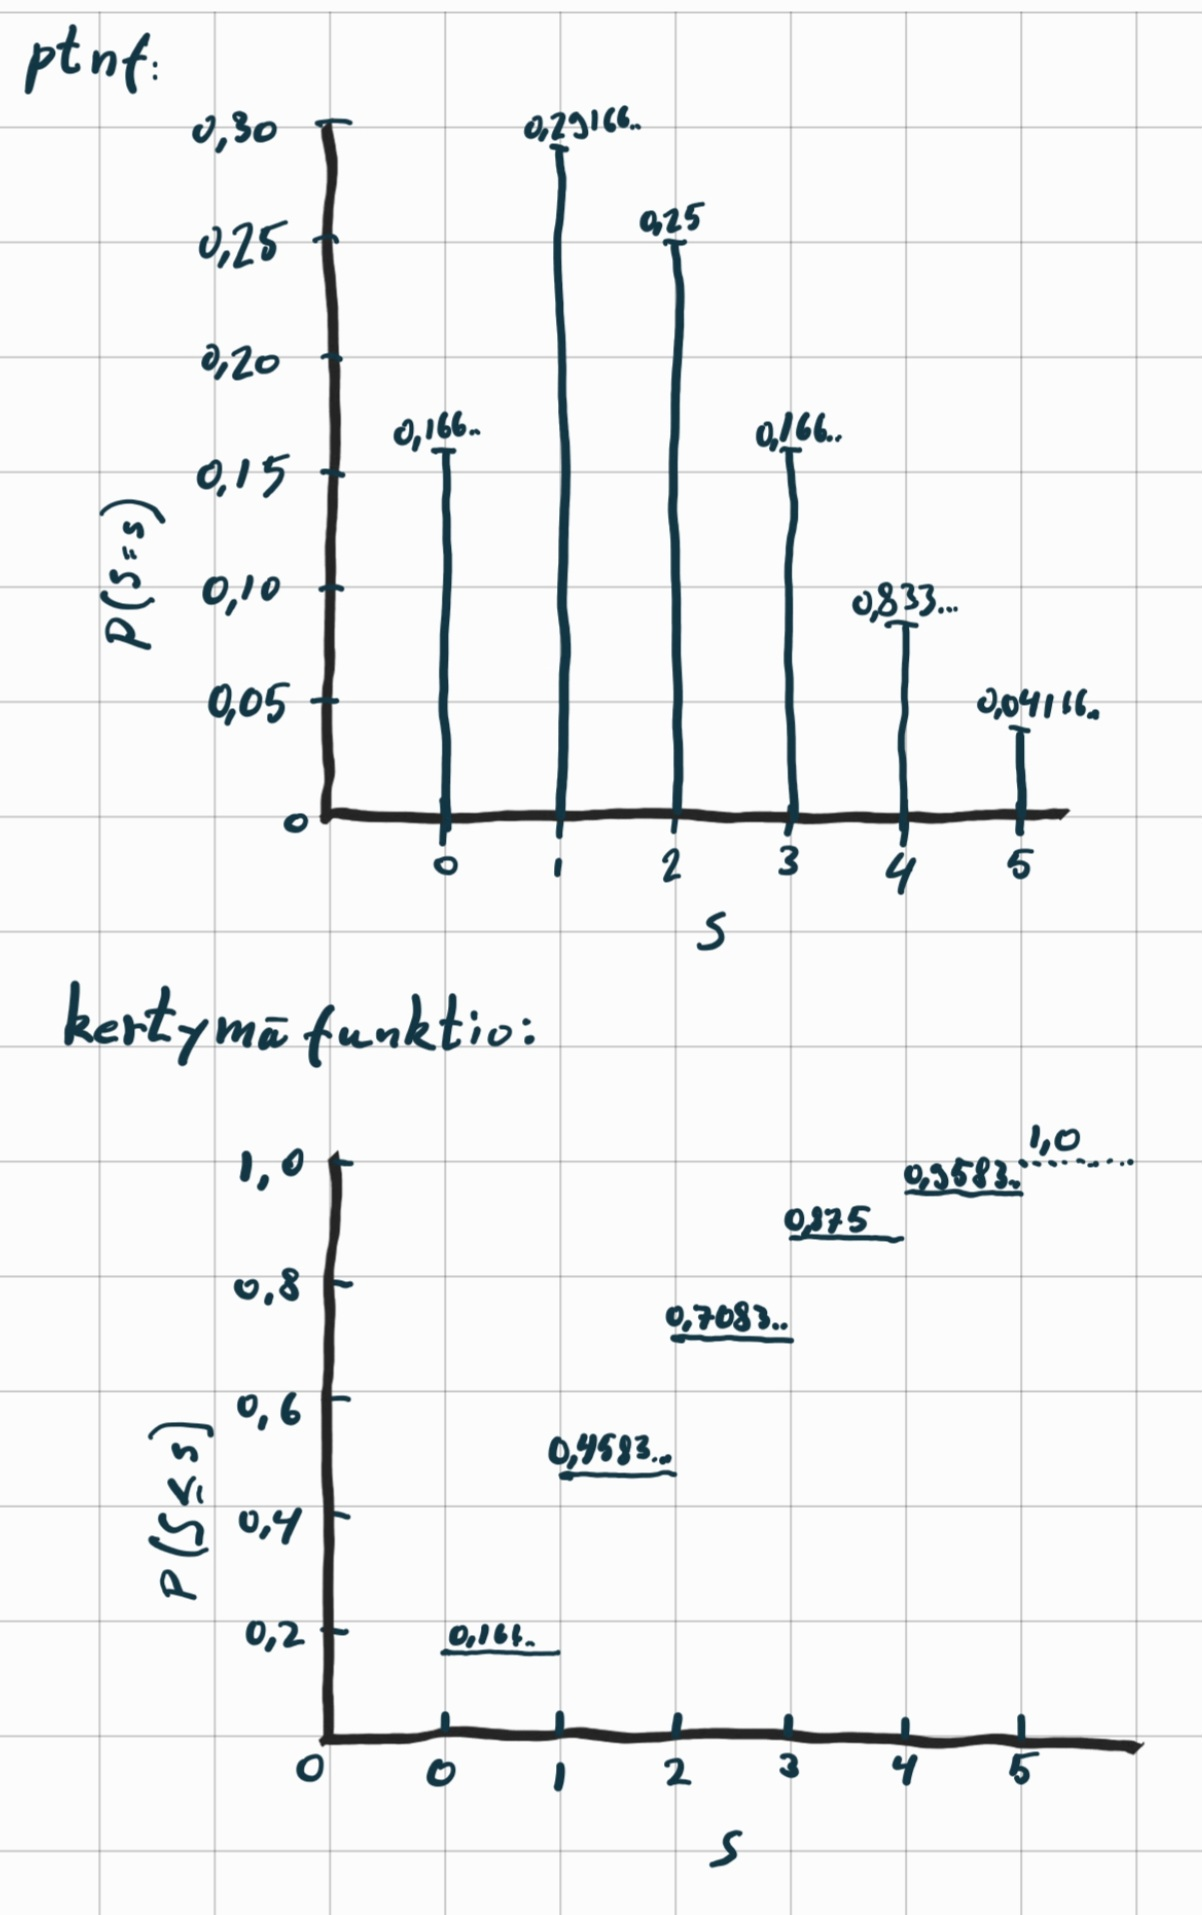
\includegraphics[width=.6\textwidth]{viikko3tehtävä5.jpg}
%  \caption{ptnf $p_S(s)=P(S=s)$}
\end{figure}






\pagebreak

\end{document}